\documentclass[11pt]{article}

\usepackage{amsmath}
\usepackage{amssymb}

\usepackage{graphicx}
\usepackage{tikz}

\usepackage{ytableau}

\title{Walks and circuits, \\ Math 4707, Spring 2021}
\date{}

\begin{document}


\maketitle

\thispagestyle{empty}

\vspace{-0.6in}


An \emph{Eulerian walk} in a graph $G$ is a walk that crosses each edge exactly once. An \emph{Eulerian circuit} is an Eulerian walk that's a circuit (a closed walk).

\begin{enumerate}

\item For each of the following graphs: does the graph have an Eulerian walk? Does it have an Eulerian circuit?
\[ (a) 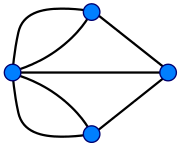
\includegraphics[width=1in]{konigsberg.png} \qquad \qquad (b) 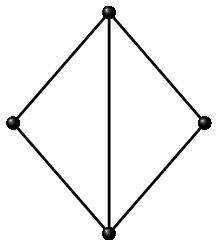
\includegraphics[width=0.8in]{kite.png} \qquad \qquad (c) 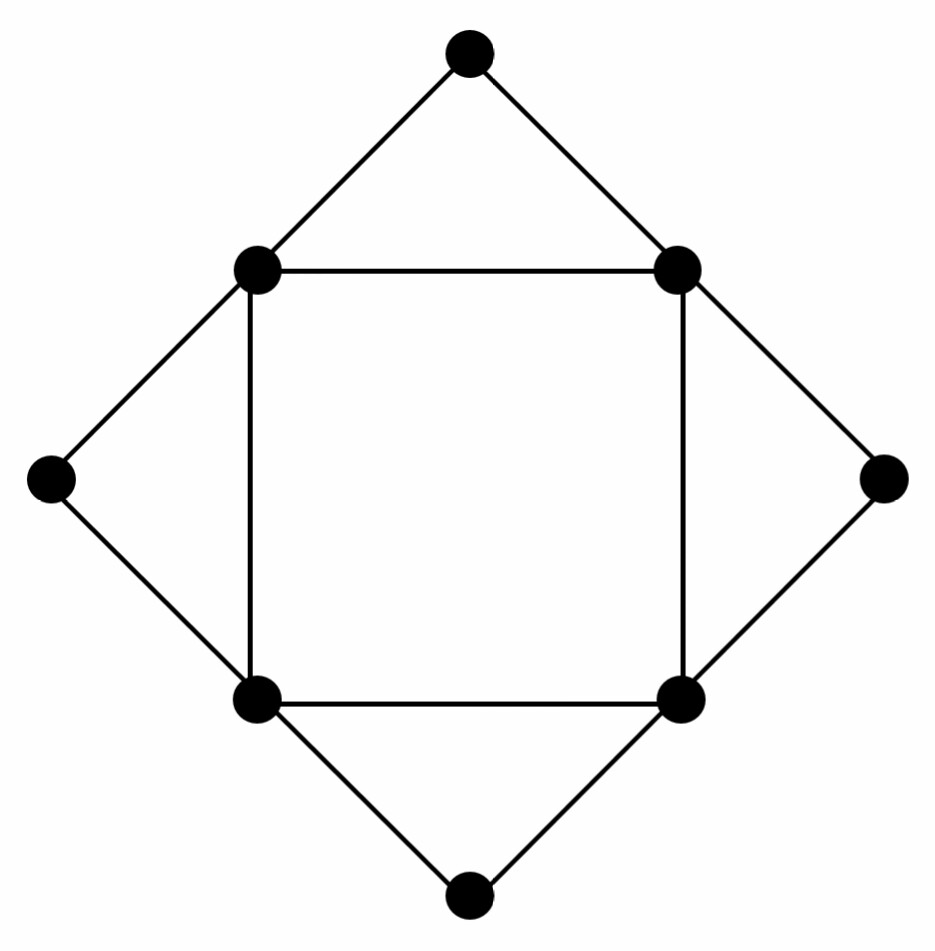
\includegraphics[width=1in]{eulerian.png} \]

\end{enumerate}

A \emph{Hamiltonian path} in a graph $G$ is a path that visits every vertex exactly once. A \emph{Hamiltonian cycle} in a graph $G$ is a cycle that visits every vertex exactly once, except that, being a cycle, it ends at the vertex it starts at.

\begin{enumerate}

\setcounter{enumi}{1}

\item For each of the following graphs: does the graph have a Hamiltonian path? Does it have a Hamiltonian cycle?
\[ (a) 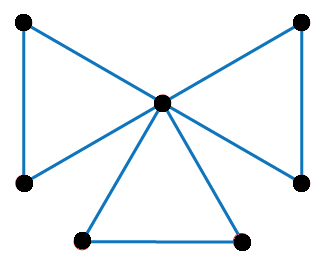
\includegraphics[width=1in]{nonhamilton.png} \qquad \qquad (b) 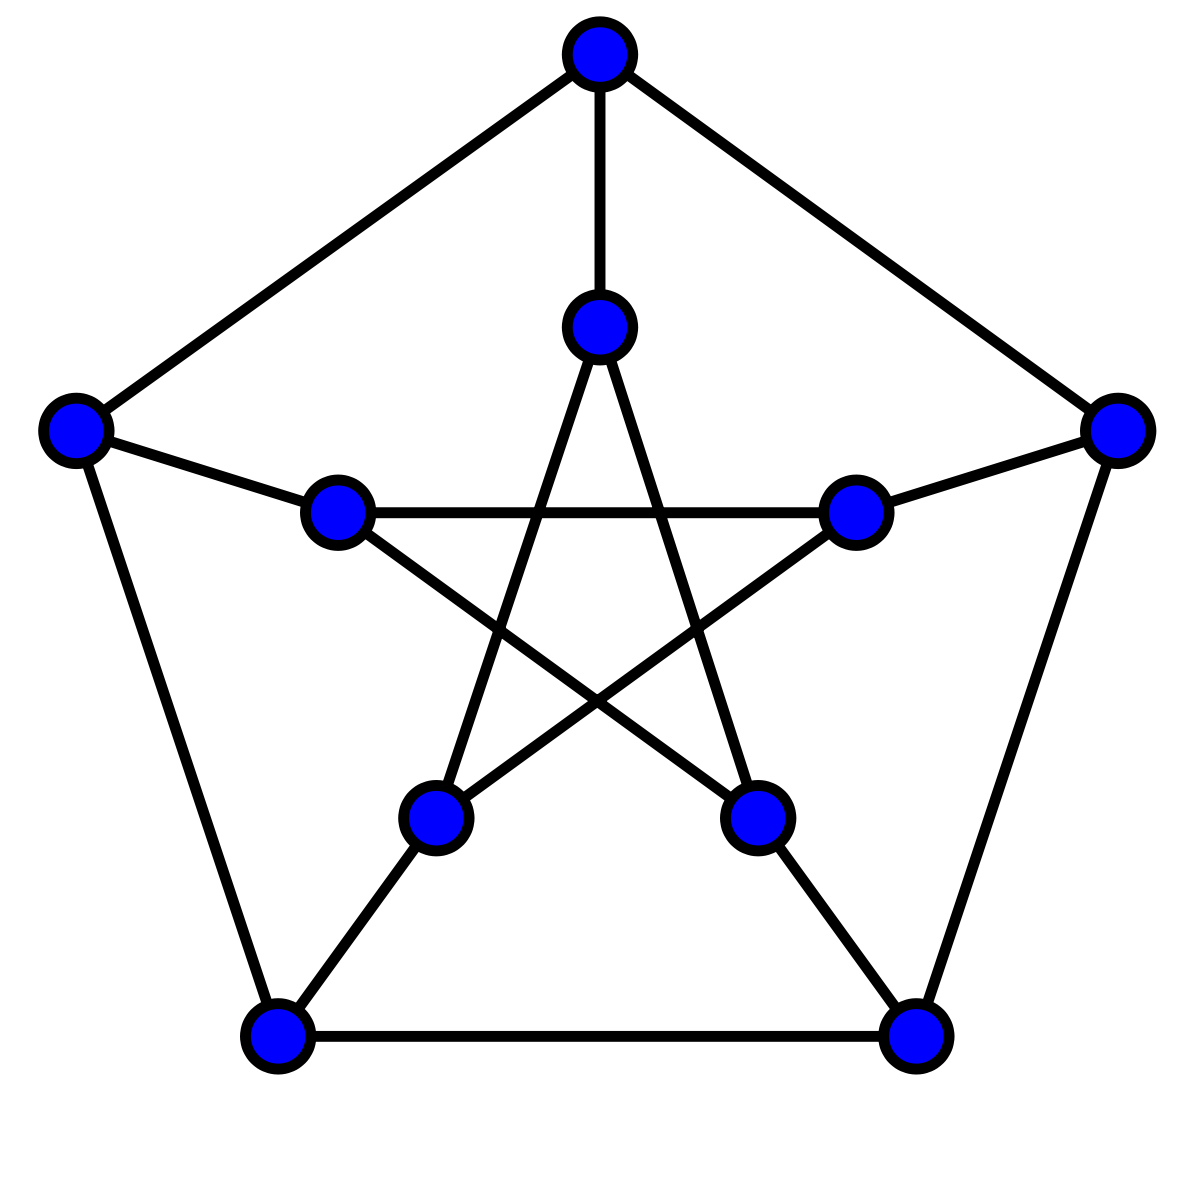
\includegraphics[width=1.1in]{petersen.png} \qquad \qquad (c) 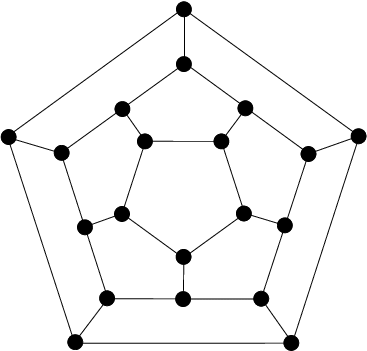
\includegraphics[width=1.1in]{dodecahedron.png}  \]



\setcounter{enumi}{2}
\item Let $G$ be a connected graph. Fill in the blanks:
\begin{itemize}
\item If $G$ has $0$ vertices with odd degree, then it has an  \rule{2cm}{0.15mm}.
\item If $G$ has exactly $2$ vertices with odd degree, then it has an \rule{2cm}{0.15mm} but not an  \rule{2cm}{0.15mm}.
\item If $G$ has more than $2$ vertices with odd degree, then it doesn't even have an \rule{2cm}{0.15mm}.
\end{itemize}
Explain why these $3$ cases cover all the possibilities for the number of odd degree vertices in a graph $G$.
\end{enumerate}

\end{document}
